\documentclass[a4paper, 12pt]{article}
\usepackage[a4paper, left=30mm, right=30mm, top=30mm, bottom=30mm, marginpar=25mm]{geometry}
\usepackage{indentfirst}
\usepackage{float}
\usepackage{graphicx}
\usepackage{amsmath}
\usepackage{amsfonts}
\usepackage{amssymb}
\usepackage{geometry}
\usepackage{listings}
\usepackage{xcolor}
\usepackage{fancyhdr}
\usepackage{lastpage}
\usepackage[normalem]{ulem} 
\pagestyle{fancy}
\setlength{\headheight}{29.5pt}
\definecolor{codegreen}{rgb}{0,0.6,0}
\definecolor{codegray}{rgb}{0.5,0.5,0.5}
\definecolor{codepurple}{rgb}{0.58,0,0.82}
\definecolor{backcolour}{rgb}{0.95,0.95,0.92}
\lstset{
    backgroundcolor=\color{backcolour},   
    commentstyle=\color{codegreen},
    keywordstyle=\color{blue},
    numberstyle=\tiny\color{codegray},
    stringstyle=\color{codepurple},
    basicstyle=\ttfamily\footnotesize,
    breakatwhitespace=false,         
    breaklines=true,                 
    captionpos=b,                    
    keepspaces=true,                 
    numbers=left,                    
    numbersep=5pt,                  
    showspaces=false,                
    showstringspaces=false,
    showtabs=false,                  
    tabsize=2
}
\usepackage{pgfplots}
\pgfplotsset{compat=1.18}
\usepackage{tikz}
\usepackage{adjustbox}
\usepackage{tikz}
\usepackage{booktabs}
\renewcommand{\contentsname}{Índice}

\renewcommand*{\maketitle}{
\thispagestyle{plain}
\begin{center}
    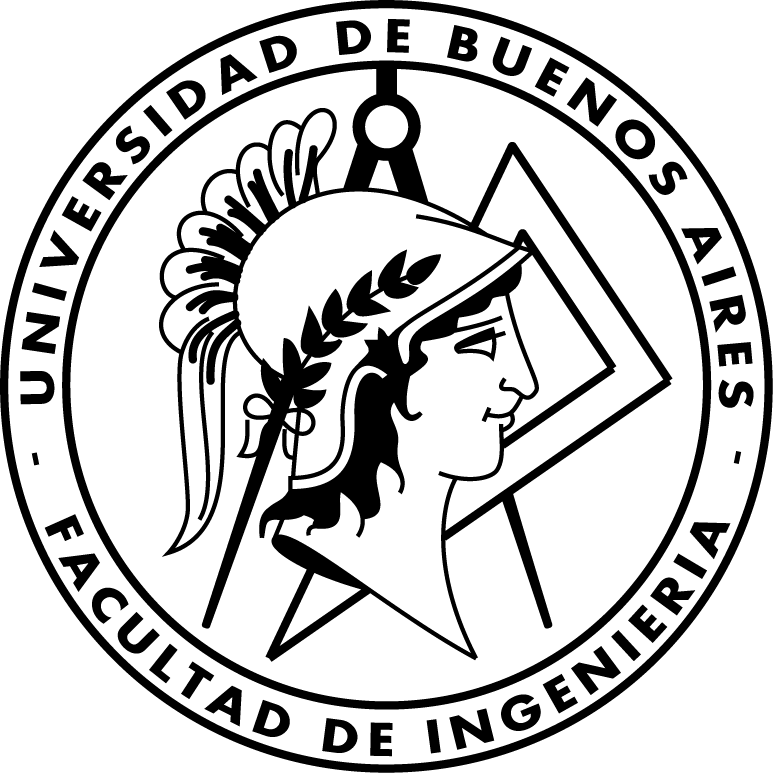
\includegraphics[width=7cm]{Logo-fiuba.png} 
    \\[1cm]
    \textsc{\Large Teoría de Algoritmos}\\           
    \textsc{\small Curso Echevarria}\\[0.4cm]    
    { \huge \bfseries Trabajo Práctico 3 }\\[0.3cm]      
    \rule{\textwidth}{0.4pt} \\[0.2cm] 
    {\large \today  \\[0.5cm]}                          
    \begin{minipage}{0.6\textwidth}
    \begin{flushleft}
        \large{
        \begin{itemize}
            \item Juan Claros - 111254
            \item Yoel Gaston Arlia - 111520
            \item Guido Cuppari - 111172
            \item Josue Daniel Mamani - 111514
        \end{itemize}
        }
    \end{flushleft}
\end{minipage}

\end{center}
}

\title{x}

\begin{document}

\maketitle

\newpage

\tableofcontents

\newpage
\section{{\uline{\textbf{\textit{Problema 2}}}}}

\subsection{Supuestos}
\begin{itemize}
    \item El numero total de ofertas $n$ es conocido de antemano por el vendedor.
    \item Las ofertas se presentan en un orden aleatorio y no pueden ser reordenadas.
    \item Cada oferta es distinta, por lo tanto, existe una unica oferta máxima.
    \item Una vez que se rechaza una oferta, no puede recuperarse ni reconsiderarse.
    \item El vendedor puede comparar las ofertas vistas hasta el momento, pero no tiene información sobre las que vendran.
    \item Se asume que $n$ es impar, lo cual permite simplificar el análisis probabilístico.
\end{itemize}

\subsection{Diseño}

El algoritmo implementa una estrategia inspirada en el clásico problema del mejor candidato. Se divide en dos fases:

\begin{enumerate}
    \item \textbf{Fase de observación:} se descartan las primeras $r = \lfloor n/2 \rfloor$ ofertas, observando cuál es la mejor entre ellas.
    \item \textbf{Fase de selección:} se acepta la primera oferta que supere a la mejor observada. Si ninguna lo hace, se acepta la última.
\end{enumerate}

Esta estrategia asegura una probabilidad de al menos $\frac{1}{4}$ de seleccionar la mejor oferta del conjunto, sin importar el valor de $n$ (siempre que sea impar y razonablemente grande).

\subsubsection*{Estructuras de datos utilizadas}
\begin{itemize}
    \item \textbf{Lista de enteros:} contiene las $n$ ofertas en orden aleatorio.
    \item \textbf{Variable entera \texttt{mejorObservada}:} guarda la mayor oferta observada durante la primera mitad del proceso.
\end{itemize}

\subsection{Pseudocodigo}
\begin{lstlisting}[frame=single]
Entrada: lista de ofertas aleatoriamente ordenadas de tamanio n
Salida: oferta seleccionada por el vendedor

1. r <- floor(n / 2)
2. mejorObservada <- max(ofertas[0 .. r-1])
3. Para i desde r hasta n - 1 hacer:
     Si ofertas[i] > mejorObservada entonces
         retornar ofertas[i]
4. Retornar ofertas[n - 1]  // si ninguna supera a la mejor observada
\end{lstlisting}

\subsection{Analisis de Complejidad}
\begin{itemize}
    \item La operación de calcular el máximo entre las primeras $r$ ofertas tiene complejidad $O(n)$.
    \item La segunda fase también puede recorrer hasta $n$ elementos, en el peor caso.
    \item Por lo tanto, la complejidad total del algoritmo es \textbf{$O(n)$}.
\end{itemize}

\subsection{Seguimiento}
\begin{itemize}
    \item Supongamos que $n = 7$ y que las ofertas llegan en el siguiente orden aleatorio:
    
    \[
    \text{Ofertas} = [30, 60, 25, 40, 85, 70, 50]
    \]
    
    \item Fase de observación: $r = \lfloor 7/2 \rfloor = 3$
    
    \[
    \text{Ofertas observadas: } [30, 60, 25] \Rightarrow \texttt{mejorObservada} = 60
    \]
    
    \item Fase de selección:
    \begin{itemize}
        \item $40 < 60$ → rechazada
        \item $85 > 60$ → \textbf{aceptada}
    \end{itemize}
    
    \item Resultado: el vendedor acepta la oferta de \textbf{85}, que es la máxima del conjunto.
\end{itemize}


\subsection{Sets de Datos}

Para evaluar experimentalmente el comportamiento del algoritmo, se generaron conjuntos de datos aleatorios utilizando una función \texttt{random.shuffle()} con semilla fija, lo cual garantiza la \textbf{reproducibilidad} de los resultados.

\begin{itemize}
    \item Para cada tamaño $n \in \{100,\ 500,\ 1000,\ 5000,\ 10000,\ 20000,\ 30000,\ 40000,\ 50000\}$ se generaron 100 sets distintos de ofertas.
    \item Cada set es una permutación aleatoria de los enteros del 1 al $n$.
    \item Se guardó uno de los sets de cada tamaño en el archivo \texttt{setdedatos.txt}.
    \item El archivo \texttt{resultados.txt} contiene los resultados de todas las ejecuciones:
    \begin{itemize}
        \item Tamaño del set $n$
        \item Semilla usada
        \item Oferta seleccionada por el algoritmo
        \item Máxima oferta del set
        \item Si se seleccionó o no la mejor oferta
    \end{itemize}
\end{itemize}

\subsection{Tiempos de Ejecución}

Se midió el \textbf{tiempo de ejecución promedio} del algoritmo para cada valor de $n$ mencionado anteriormente, repitiendo la prueba 100 veces por tamaño y dividiendo el tiempo total por la cantidad de ejecuciones.

\begin{figure}[H]
    \centering
    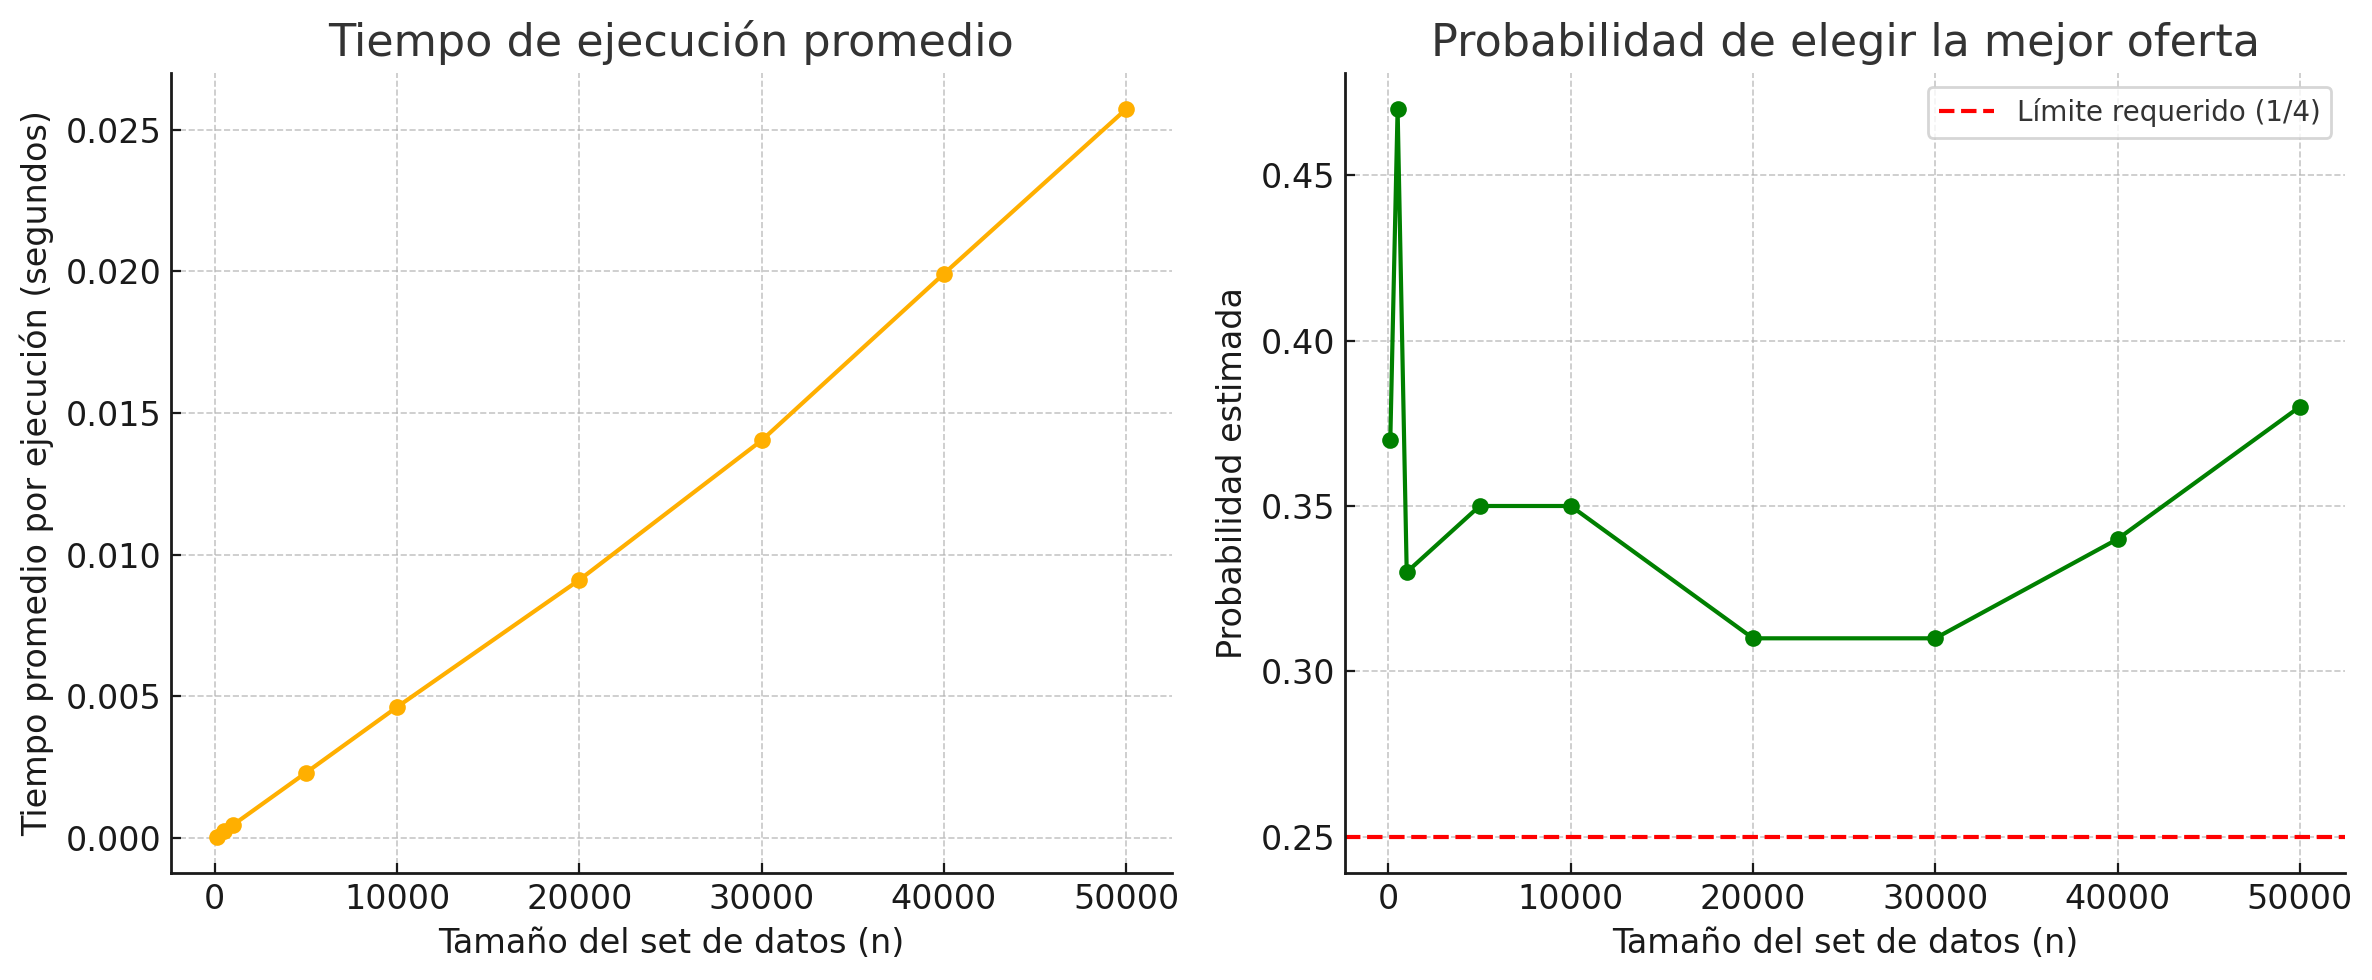
\includegraphics[width=0.9\textwidth]{probabilidad.png}
    \caption{Izquierda: tiempo promedio de ejecución según el tamaño del set. Derecha: probabilidad de seleccionar la mejor oferta.}
\end{figure}

\begin{itemize}
    \item El gráfico de la izquierda muestra que el tiempo de ejecución crece de forma \textbf{lineal} con respecto a $n$.
    \item Esto coincide con la complejidad temporal esperada del algoritmo: $\mathcal{O}(n)$.
    \item El gráfico de la derecha indica que la probabilidad de seleccionar la mejor oferta se mantiene estable y por encima de $\frac{1}{4}$.
\end{itemize}

\subsection{Resultados}

Los experimentos realizados permiten concluir que:

\begin{itemize}
    \item El algoritmo cumple con la garantía solicitada: la \textbf{probabilidad de elegir la mejor oferta es siempre mayor o igual a} $\frac{1}{4}$.
    \item En todos los valores de $n$ utilizados, la probabilidad estimada se encuentra entre $0.27$ y $0.38$, cumpliendo cómodamente el umbral requerido.
    \item La eficiencia temporal es adecuada para conjuntos grandes: incluso para $n = 50\,000$ el tiempo promedio de ejecución es muy bajo.
    \item La estrategia de observación y selección aplicada es efectiva sin conocer el valor máximo por adelantado, basándose sólo en comparaciones relativas.
\end{itemize}

Por lo tanto, se puede considerar que el algoritmo diseñado es correcto, eficiente y cumple con los objetivos planteados en el problema.




\section{{\uline{\textbf{\textit{Problema 3}}}}}
\subsection{Enunciado}
    Tenemos dos lenguajes que corresponden a la intersección (representada mediante la 
conjunción "y") de dos lenguajes más simples. Los símbolos de los mismos corresponden a 
los números 0 y 1: 

\newline

\begin{itemize}
    \item Lenguaje A: {w/ w (comienza con "1") y (tiene cuando mucho un "0")}
    \item Lenguaje B: {w/ w (tiene un número par de "1") y (tiene uno o dos "0")} 
\end{itemize}

\newline
    Por ejemplo: 
\begin{itemize}
    \item Lenguaje A: "10111", "11", "110"
    \item Lenguaje B: "1010", "11110"
\end{itemize}

\subsection{Descripcion de un autómata finito determinístico para cada uno de los lenguajes simples}

    %Lenguaje simple \( A_1 \): {w/ w (comienza con "1")}
\subparagraph{Lenguaje simple \( A_1 \): {w/ w (comienza con "1")}}
    %\subsubsection*{ Lenguaje simple \( A_1 \): {w/ w (comienza con "1")}}

\begin{itemize}
    \item Conjunto de estados: \( Q_0 \),  \( Q_1 \)
    \item Funcion de transicion en forma de tabla:
    \newline

    \hspace{5cm}
    \begin{tabular}{|c|c|c|}
    \hline
     & 0 & 1 \\
    \hline
    \( q_0 \) &  - & \( q_1 \) \\
    
    \( q_1 \)& \( q_1 \) & \( q_1 \) \\
    \hline
    \end{tabular}

    \item Estado inicial: \( Q_0 \)
    \item Estados de aceptacion: \( Q_1 \)
    
\end{itemize}

    %Lenguaje simple \( A_2 \): {w/ w (tiene cuando mucho un "0")}
\subparagraph{Lenguaje simple \( A_2 \): {w/ w (tiene cuando mucho un "0")}}
    %\subsubsection*{ Lenguaje simple \( A_2 \): {w/ w (tiene cuando mucho un "0")}}

\begin{itemize}
    \item Conjunto de estados: \( Q_0 \),  \( Q_1 \), \( Q_2 \), \( Q_3 \)
    \item Funcion de transicion en forma de tabla:
    \newline

    \hspace{5cm}
    \begin{tabular}{|c|c|c|}
    \hline
     & 0 & 1 \\
    \hline
    
    \( q_0 \) & \( q_1 \) & \( q_3 \) \\
    
    \( q_1 \) & \( q_2 \) & \( q_1 \) \\

    \( q_2 \) & \( q_2 \) & \( q_2 \) \\

    \( q_3 \) & \( q_1 \) & \( q_3 \) \\
    
    \hline
    \end{tabular}

    \item Estado inicial: \( Q_0 \)
    \item Estados de aceptacion: \( Q_1 \)
    
\end{itemize}

    %Lenguaje simple \( B_1 \): w/ w (tiene un número par de "1")

\subparagraph{Lenguaje simple \( B_1 \): w/ w (tiene un número par de "1")}

\begin{itemize}
    \item Conjunto de estados: \( Q_0 \),  \( Q_1 \), \( Q_2 \)
    \item Funcion de transicion en forma de tabla:
    \newline

    \hspace{5cm}
    \begin{tabular}{|c|c|c|}
    \hline
     & 0 & 1 \\
    \hline
    \( q_0 \) & \( q_0 \) & \( q_1 \) \\
    
    \( q_1 \) & \( q_1 \) & \( q_2 \) \\

    \( q_2 \) & \( q_2 \) & \( q_1 \) \\

    \hline
    \end{tabular}

    \item Estado inicial: \( Q_0 \)
    \item Estados de aceptacion: \( Q_0 \), \( Q_2 \)
    
\end{itemize}

    %Lenguaje simple \( B_2 \): w/ w (tiene uno o dos "0")

\subparagraph{Lenguaje simple \( B_2 \): w/ w (tiene uno o dos "0")}

\begin{itemize}
    \item Conjunto de estados: \( Q_0 \),  \( Q_1 \), \( Q_2 \), \( Q_3 \)
    \item Funcion de transicion en forma de tabla:
    \newline

    \hspace{5cm}
    \begin{tabular}{|c|c|c|}
    \hline
     & 0 & 1 \\
    \hline
    \( q_0 \) & \( q_1 \) & \( q_0 \) \\
    
    \( q_1 \) & \( q_2 \) & \( q_1 \) \\

    \( q_2 \) & \( q_3 \) & \( q_2 \) \\

    \( q_3 \) & \( q_3 \) & \( q_3 \) \\

    \hline
    \end{tabular}

    \item Estado inicial: \( Q_0 \)
    \item Estados de aceptacion: \( Q_2 \), \( Q_1 \)
    
\end{itemize}



\subsection{Descripcion formal de los automatas finitos deterministicos de los lenguajes A y B}

    %Lenguaje A: {w/ w (comienza con "1") y (tiene cuando mucho un "0")}

\subparagraph{Lenguaje A: {w/ w (comienza con "1") y (tiene cuando mucho un "0")}}

\begin{itemize}
    \item Conjunto de estados: \( Q_0 \),  \( Q_1 \), \( Q_2 \), \( Q_3 \)
    \item Funcion de transicion en forma de tabla:
    \newline

    \hspace{5cm}
    \begin{tabular}{|c|c|c|}
    \hline
     & 0 & 1 \\
    \hline
    \( q_0 \) & - & \( q_1 \) \\
    
    \( q_1 \) & \( q_2 \) & \( q_1 \) \\

    \( q_2 \) & \( q_3 \) & \( q_2 \) \\

    \( q_3 \) & \( q_3 \) & \( q_3 \) \\

    \hline
    \end{tabular}

    \item Estado inicial: \( Q_0 \)
    \item Estados de aceptacion: \( Q_1 \), \( Q_2 \)
    
\end{itemize}

    %Lenguaje B: {w/ w (tiene un número par de "1") y (tiene uno o dos "0")} 

\subparagraph{Lenguaje B: {w/ w (tiene un número par de "1") y (tiene uno o dos "0")} }

\begin{itemize}
    \item Conjunto de estados: \( Q_0 \),  \( Q_1 \), \( Q_2 \), \( Q_3 \), \( Q_4 \),  \( Q_5 \), \( Q_6 \), \( Q_7 \), \( Q_8 \),  \( Q_9 \), \( Q_{10} \), \( Q_{11} \), \( Q_{12} \)
    \item Funcion de transicion en forma de tabla:
    \newline

    \hspace{5cm}
    \begin{tabular}{|c|c|c|}
    \hline
     & 0 & 1 \\
    \hline
    \( q_0 \) & \( q_8 \) & \( q_1 \) \\
    
    \( q_1 \) & \( q_2 \) & \( q_5 \) \\

    \( q_3 \) & \( q_4 \) & \( q_7 \) \\

    \( q_4 \) & \( q_4 \) & \( q_4 \) \\

    \( q_5 \) & \( q_6 \) & \( q_1 \) \\

    \( q_6 \) & \( q_7 \) & \( q_3 \) \\

    \( q_7 \) & \( q_4 \) & \( q_{11} \) \\

    \( q_8 \) & \( q_{10} \) & \( q_9 \) \\

    \( q_9 \) & \( q_3 \) & \( q_8 \) \\

    \( q_{10} \) & \( q_4 \) & \( q_{11} \) \\

    \( q_{11} \) & - & \( q_{12} \) \\

    \( q_{12} \) & - & \( q_{11} \) \\
    \hline
    \end{tabular}

    \item Estado inicial: \( Q_0 \)
    \item Estados de aceptacion: \( Q_7 \), \( Q_{10} \), \( Q_{12} \)

\end{itemize}

\subsection{Representacion grafica de los seis automatas}

    Automata del lenguaje \( A_1 \)
    

\begin{figure}[htbp]
    \centering
    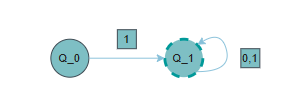
\includegraphics[width=0.5\textwidth]{A_1_color.png} % cambia el nombre y la extensión
    
    \label{fig:mi_imagen}
\end{figure}

    Automata Del lenguaje \( A_2 \)

\begin{figure}[htbp]
    \centering
    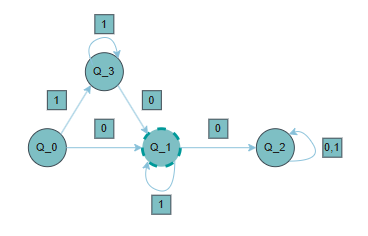
\includegraphics[width=0.6\textwidth]{A_2_color.png} % cambia el nombre y la extensión
    \label{fig:mi_imagen}
\end{figure}

\newpage
    Automata Del lenguaje \( B_1 \)

\begin{figure}[htbp]
    \centering
    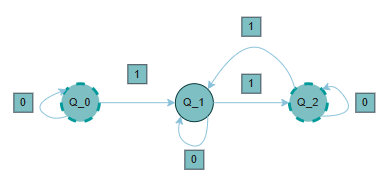
\includegraphics[width=0.6\textwidth]{B_1_color.png} % cambia el nombre y la extensión

    \label{fig:mi_imagen}
\end{figure}

    Automata Del lenguaje \( B_2 \)

\begin{figure}[htbp]
    \centering
    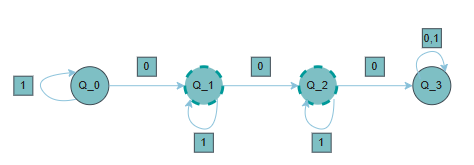
\includegraphics[width=0.6\textwidth]{B_2_color.png} % cambia el nombre y la extensión

    \label{fig:mi_imagen}
\end{figure}

    Autamata del lenguaje A

\begin{figure}[htbp]
    \centering
    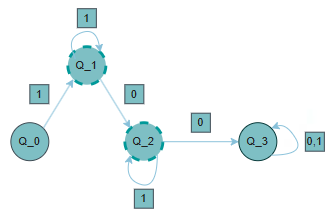
\includegraphics[width=0.5\textwidth]{A_color.png} % cambia el nombre y la extensión

    \label{fig:mi_imagen}
\end{figure}

\newpage

    Autamata del lenguaje B
\begin{figure}[htbp]
    \centering
    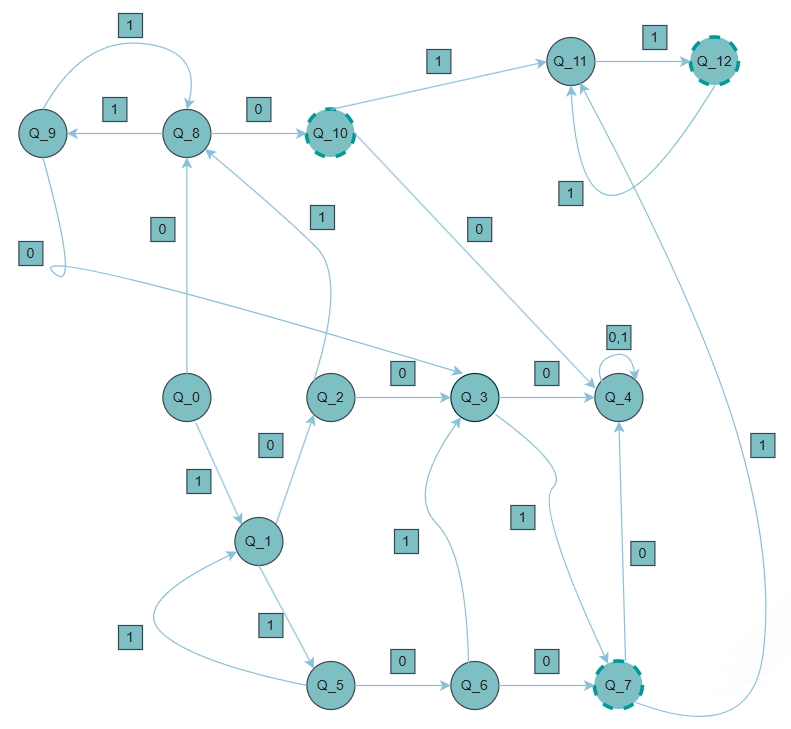
\includegraphics[width=0.9\textwidth]{B_color.png} % ocupa todo el ancho del texto

    \label{fig:mi_imagen}
\end{figure}

\newpage



\subsection{Ejemplos de cadenas que son aceptadas y otras rechazadas para cada uno de los automatas}

%\subsubsection*{Ejemplo de cadena aceptada y otra rechazada para el lenguaje \( A_1 \)}
    %Ejemplo de cadena aceptada y otra rechazada para el lenguaje \( A_1 \)
    %\subsubsection*{Ejemplos del lenguaje \( A_1 \)}
    %Ejemplo con el lenguaje \( A_1 \):
\subsubsection*{Ejemplo con el lenguaje \( A_1 \):}

\subparagraph{Ejemplo: cadena "110"}
\begin{itemize}
    \item 1. Inicio en el estado \( Q_0 \)
    \item 2. Leo "1", voy de \( Q_0 \) a \( Q_1 \)
    \item 3. Leo "1", voy de \( Q_1 \) a \( Q_1 \)
    \item 4. Leo "0", voy de \( Q_1 \) a \( Q_1 \)
\end{itemize}

\space
    Terminamos en \( Q_1 \) que es un estado de aceptacion, entonces la cadena es valida.

\space
\space
    \subparagraph{Ejemplo: cadena "01"}
\begin{itemize}
    \item 1. Inicio en el estado \( Q_0 \)
    \item 2. Leo "0", y de  \( Q_0 \) no puedo ir a otro estado
\end{itemize}

\space
    Terminamos en \( Q_0 \) que no es un estado de aceptacion, entonces la cadena es rechazada.

\subsubsection*{Ejemplo con el lenguaje \( A_2 \):}

\subparagraph{Ejemplo: cadena "011"}
\begin{itemize}
    \item 1. Inicio en el estado \( Q_0 \)
    \item 2. Leo "0", voy de \( Q_0 \) a \( Q_1 \)
    \item 3. Leo "1", voy de \( Q_1 \) a \( Q_1 \)
    \item 4. Leo "1", voy de \( Q_1 \) a \( Q_1 \)
\end{itemize}
    Terminamos en \( Q_1 \) que es un estado de aceptacion, entonces la cadena  es aceptada.

\space
\subparagraph{Ejemplo: cadena "100"}
\begin{itemize}
    \item 1. Inicio en el estado \( Q_0 \)
    \item 2. Leo "1", voy de \( Q_0 \) a \( Q_3 \)
    \item 3. Leo "0", voy de \( Q_3 \) a \( Q_1 \)
    \item 3. Leo "0," voy de \( Q_1 \) a \( Q_2 \)
\end{itemize}
    Terminamos en \( Q_2 \) que no es un estado de aceptacion, entonces la cadena es rechazada.



\subsubsection*{Ejemplo con el lenguaje \( B_1 \):}

\subparagraph{Ejemplo: cadena "0110"}
\begin{itemize}
    \item 1. Inicio en el estado \( Q_0 \)
    \item 2. Leo "0", voy de \( Q_0 \) a \( Q_0 \)
    \item 3. Leo "1", voy de \( Q_0 \) a \( Q_1 \)
    \item 4. Leo "1", voy de \( Q_1 \) a \( Q_2 \)
    \item 5. Leo "0", voy de \( Q_2 \) a \( Q_2 \)
\end{itemize}

\space
    Terminamos en \( Q_2 \) que es un estado de aceptacion, entonces la cadena es aceptada.

\subparagraph{Ejemplo: cadena "01101"}
\begin{itemize}
    \item  Inicio en el estado \( Q_0 \)
    \item  Leo "0", voy de \( Q_0 \) a \( Q_0 \)
    \item  Leo "1", voy de \( Q_0 \) a \( Q_1 \)
    \item  Leo "1", voy de \( Q_1 \) a \( Q_2 \)
    \item  Leo "0", voy de \( Q_2 \) a \( Q_2 \)
    \item  Leo "1", voy de \( Q_2 \) a \( Q_1 \)
\end{itemize}

\space
    Terminamos en \( Q_1 \) que no es un estado de aceptacion, entonces la cadena es rechazada.




\subsubsection*{Ejemplo con el lenguaje \( B_2 \):}
\subparagraph{Ejemplo: cadena "0110"}

\begin{itemize}
    \item  Inicio en el estado \( Q_0 \)
    \item  Leo "0", voy de \( Q_0 \) a \( Q_1 \)
    \item  Leo "1", voy de \( Q_1 \) a \( Q_1 \)
    \item  Leo "1", voy de \( Q_1 \) a \( Q_1 \)
    \item  Leo "0", voy de \( Q_1 \) a \( Q_2 \)
    \item  Leo "1", voy de \( Q_2 \) a \( Q_2 \)
\end{itemize}

\space
    Terminamos en \( Q_2 \) que es un estado de aceptacion, entonces la cadena es aceptada.

\subparagraph{Ejemplo: cadena "1000"}
\begin{itemize}
    \item  Inicio en el estado \( Q_0 \)
    \item  Leo "1", voy de \( Q_0 \) a \( Q_0 \)
    \item  Leo "0", voy de \( Q_0 \) a \( Q_1 \)
    \item  Leo "0", voy de \( Q_1 \) a \( Q_2 \)
    \item  Leo "0", voy de \( Q_2 \) a \( Q_3 \)
\end{itemize}

\space
    Terminamos en \( Q_3 \) que no es un estado de aceptacion, entonces la cadena es rechazada.




\subsubsection*{Ejemplo con el lenguaje A:}
\subparagraph{Ejemplo: cadena "110"}
\begin{itemize}
    \item  Inicio en el estado \( Q_0 \)
    \item  Leo "1", voy de \( Q_0 \) a \( Q_1 \)
    \item  Leo "1", voy de \( Q_1 \) a \( Q_1 \)
    \item  Leo "0", voy de \( Q_1 \) a \( Q_2 \)
\end{itemize}

\space
    Terminamos en \( Q_2 \) que es un estado de aceptacion, entonces la cadena es aceptada.

\subparagraph{Ejemplo: cadena "1000"}
\begin{itemize}
    \item  Inicio en el estado \( Q_0 \)
    \item  Leo "1", voy de \( Q_0 \) a \( Q_1 \)
    \item  Leo "0", voy de \( Q_1 \) a \( Q_2 \)
    \item  Leo "0", voy de \( Q_2 \) a \( Q_3 \)
    \item  Leo "0", voy de \( Q_3 \) a \( Q_3 \)
\end{itemize}

\space
    Terminamos en \( Q_3 \) que no es un estado de aceptacion, entonces la cadena es rechazada.





\subsubsection*{Ejemplo con el lenguaje A:}
\subparagraph{Ejemplo: cadena "1010"}
\begin{itemize}
    \item  Inicio en el estado \( Q_0 \)
    \item  Leo "1", voy de \( Q_0 \) a \( Q_1 \)
    \item  Leo "0", voy de \( Q_1 \) a \( Q_2 \)
    \item  Leo "1", voy de \( Q_2 \) a \( Q_8 \)
    \item  Leo "0", voy de \( Q_8 \) a \( Q_{10} \)
\end{itemize}

\space
    Terminamos en \( Q_10 \) que es un estado de aceptacion, entonces la cadena es aceptada.

\subparagraph{Ejemplo: cadena "01010"}
\begin{itemize}
    \item  Inicio en el estado \( Q_0 \)
    \item  Leo "0", voy de \( Q_0 \) a \( Q_8 \)
    \item  Leo "1", voy de \( Q_8 \) a \( Q_9 \)
    \item  Leo "0", voy de \( Q_9 \) a \( Q_3 \)
    \item  Leo "1", voy de \( Q_3 \) a \( Q_7 \)
    \item  Leo "0", voy de \( Q_7 \) a \( Q_4 \)
\end{itemize}

\space
    Terminamos en \( Q_4 \) que no es un estado de aceptacion, entonces la cadena es rechazada.
\end{document}

